% This is samplepaper.tex, a sample chapter demonstrating the
% LLNCS macro package for Springer Computer Science proceedings;
% Version 2.21 of 2022/01/12
%
\documentclass[runningheads]{llncs}
%
\usepackage[T1]{fontenc}
% T1 fonts will be used to generate the final print and online PDFs,
% so please use T1 fonts in your manuscript whenever possible.
% Other font encondings may result in incorrect characters.
%
\usepackage{graphicx}
% Used for displaying a sample figure. If possible, figure files should
% be included in EPS format.
%
% If you use the hyperref package, please uncomment the following two lines
% to display URLs in blue roman font according to Springer's eBook style:
%\usepackage{color}
%\renewcommand\UrlFont{\color{blue}\rmfamily}
%
\usepackage[ngerman]{babel}
\usepackage{wrapfig}
\begin{document}
%
\title{Gruppe 3: Catchphrase?}
%
%\titlerunning{Abbreviated paper title}
% If the paper title is too long for the running head, you can set
% an abbreviated paper title here
%
\author{...\inst{1}\and
...\inst{1}\and
...\inst{1}\and
...\inst{1}}
%
\authorrunning{F. Author et al.}
% First names are abbreviated in the running head.
% If there are more than two authors, 'et al.' is used.
%
\institute{FernUniversität in Hagen, Universitätsstraße 47, 58097 Hagen, Deutschland
\email{\{...\}@studium.fernuni-hagen.de}\\
\url{https://www.fernuni-hagen.de}}
%
\maketitle              % typeset the header of the contribution
%
%
\section{Einleitung}
TODO Gruppenbeschreibung
\section{Kommunikation und Kommunikationsmittel}
TODO Gruppentreffen, Github

\section{Technische Rahmenbedingungen und Softwarebasisarchitektur}
TODO Java, Bdi, 2 Agentensysteme, UML

\section{Gruppenbeitrag Heinz Stadler}
Nach einer ausführlichen Einarbeitung in die Thematik der Multiagentensysteme, erfolgte die Analyse der Ergebnisse des 15. Multi-Agent Programming Contest \cite{Ahlbrecht2021}. Diese ergab, dass neben der Entscheidungsfindung der Agenten, der Aufbau einer konsistenten und umfangreichen Wissensbasis (vgl. \cite[S. 29]{Ahlbrecht2021}) sowie die effiziente Problemfindung (vgl. \cite[S. 17]{Ahlbrecht2021}), eine wesentliche Schwierigkeit der Aufgabe bilden. \\
Als Folge dessen entschied sich der Autor mit dem Aufbau der Wissensverwaltung (siehe \ref{wissensverwaltung}) zu beginnen. Diese umfasst eine Datenstruktur zur Speicherung der von der Simulation übermittelten Informationen, sowie eine Lösung zum Aufbau einer globalen Karte des Simulationsgebiets. Nach Fertigstellung der Karte und deren funktionalen Verifikation, wurde parallel an der Konzeptionierung des Agentensystem V1 (siehe \ref{agentV1}) sowie der Implementierung einer intelligenten Wegführung (siehe \ref{wegfindung}) gearbeitet. Um die Ergebnisse der Wegführung und das Entscheidungsverhalten der Agenten effektiv verifizieren zu können, folgte die Erstellung eines graphischen Analysewerkzeugs (siehe \ref{verifikation}) das im weiten Entwicklungsverlauf stetig weiterentwickelt wurde und sich als sehr hilfreich bei der Fehlerfindung zeigte.
 
\subsection{Agent V1 - Architektur}\label{agentV1}
\begin{wrapfigure}{r}{0.56\linewidth}
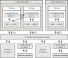
\includegraphics{./Referenzen/Architekturdiagramm.pdf}
\caption{Dummy figure.}
\label{g3:architecture}
\end{wrapfigure}
Das Agentensystem V1 wurde federführend vom Autor konzipiert, in der Gruppe abgestimmt und schließlich selbstständig implementiert. Es erweitert das BDI-Konzept \cite{Bratman1987} um zusätzliche Daten-, Berechnungs- und Entscheidungsebenen, die in Abbildung \ref{g3:architecture} illustriert sind. \\
Das System kombiniert das Konzept des BDI-Agenten mit dem Konzept einer bidirektionalen vertikalen Schichtarchitektur \cite[S. 61-62]{Weiss2000}, auf die in Abschnitt
\ref{absichtsfindung} näher eingegangen wird. \\
Jeder BDI-Agent wurde mit einer Vorgesetzteninstanz kombiniert und in einem Thread gekapselt. Die Kommunikation zwischen Agenten erfolgt über Nachrichten. Agenten können zu Agentengruppen zusammengefasst werden, welche die im Simulationsverlauf erhaltenen Umgebungsinformationen in einer gemeinsamen Karte verwalten. Die Karte und die Module zur Wegführung werden von einem zentralem Navigationsmodul, das als Einzelstück ausgeführt wurde, verwaltet. 



 Dies ermöglicht die parallelisierte Entscheidungsfindung und unterstreicht die konzeptionelle Eigenständig der Agenten untereinander. Agenten können zu Agentengruppen zusammengefasst werden. In jeder Agentengruppe bleibt der Vorgesetzte des Agenten mit der niedrigsten Index aktiv und übernimmt die Vorgesetztenrolle der anderen Agenten in der Gruppe. Die  

\subsection{Wissensverwaltung}\label{wissensverwaltung}
Belief, Karten
\\
\\
Die zur Kommunikation mit dem Simulationsserver gewählte Bibliothek EISMASSim \cite{EISMASSim} ermöglicht die Abfrage der aktuellen Simulationsinformationen in der Form von Percepts. Da Percepts eine universelle Datenstruktur, unabhängig vom jeweiligen Dateninhalt ist, wurde die Java Klasse Belief erstellt. In dieser werden die aktuellen Percepts in einfach zu verarbeitende Java Datenstrukturen umgewandelt. \\
Zusätzlich werden die aktuellen Informationen aus dem Sichtfeld der Agenten in eine weitere Datenstruktur GameMap, im Folgenden als Karte bezeichnet, gespeichert. Die Karte hat zum Ziel umfangreiches Wissen über die Umgebung der Agenten zu sammeln. Sie besteht aus einzelnen Zellen, die chronologisch Informationen der Agenten persistiert. Die Karte ermöglicht Informationen von Agenten, die nachweislich inkorrekte Daten gesendet haben, zu entfernen. Des Weiteren können verschiedene Karten zusammengeführt werden, wobei die Chronologie der enthaltenen Daten gewahrt wird. \\
Da die absolute Position der Agenten zum Simulationsbeginn nicht bekannt ist, stellt das Zusammenführen einzelner Karten eine Schwierigkeit dar. Im Nachfolgenden wird 

\subsection{Wegfindung}\label{wegfindung}
Pathfinding

\subsection{Ziel- und Absichtsfindung}\label{absichtsfindung}
Desires

\subsection{Verifikation und Problemfindung}\label{verifikation}
Tests / Debugger

\subsection{...}

\section{Gruppenbeitrag Melinda Betz}

\section{Gruppenbeitrag Phil Heger}

\section{Gruppenbeitrag Björn Wladasch}

\section{Turniere}
\subsubsection{Turnier 2}
\subsubsection{Turnier 3}
\subsubsection{Turnier 4}
\subsubsection{Turnier 5}
\subsubsection{Turnier 6}

\section{Rekapitulation und Ausblick}
Vor- und Nachteile der Entscheidung von zwei Architekturen
Was sollte noch verbessert werden
Wie sind wir zufrieden


%
% ---- Bibliography ----
%
% BibTeX users should specify bibliography style 'splncs04'.
% References will then be sorted and formatted in the correct style.
%
% \bibliographystyle{splncs04}
% \bibliography{mybibliography}
%
\begin{thebibliography}{8}
	\bibitem{Ahlbrecht2021}
	Ahlbrecht, T., Dix, J., Fiekas. N. und T. Krausburg: The Multi-Agent Programming Contest 2021, Springer, Heidelberg, 2021
	\bibitem{Hart1968}
	Hart, P. E., Nilsson, N. J. und Raphael, B.: A Formal Basis for the Heuristic Determination of Minimum Cost Paths, in IEEE Transactions on Systems Science and Cybernetics, 4. Auflage, Nummer 2, Seiten 100-107, Juli 1968
	\bibitem{Weiss2000}
	Weiss, G.: Multiagent Systems, 2. Auflage, The MIT Press, Cambridge, 2000
	\bibitem{EISMASSim}
	github.com/agentcontest/massim\_2022, agentcontest/massim\_2022, \\ https://github.com/agentcontest/massim\_2022/blob/main/docs/eismassim.md, EISMASSim Documentation, 21.08.2022
	\bibitem{Bratman1987}
	Bratman, M.: Intention, plans, and practical reason, Harvard University Press, Cambridge, 1987
\end{thebibliography}
\end{document}
